\documentclass{beamer}
\usetheme{metropolis}
\usepackage{pgfpages}
\usepackage{listings}

\ifdefined\NOTES
  \setbeameroption{show only notes}
\fi

\title[Devops Series]{Devops in a nutshell}
\author{Kevin Wang}
\year=2019\relax
\month=05\relax
\day=02\relax
\date{\today}
\institute{DevX}
\logo{
\includegraphics[height=0.5cm]{assets/devxlogo.png}}

\begin{document}

\maketitle

\section{Introduction}

\begin{frame}{What is devops?}
  \pause
  \begin{center}
    a set of application development and operations practices to release
    software
  \end{center}
\end{frame}
\note[itemize]{
  \item application development and operations used to be more segregated
  \item faster paced environment necessitates closer interaction between
    development and operations
  \item devops is a set of practices of developing, testing, deploying, and
    monitoring software to release it at a faster rate
}

\begin{frame}{whoami}
  \textbf{\Large Kevin Wang}

  Tech evangelist

  \begin{description}
    \item[LA Hacks] Tech Director Emeritus
    \item[DevX] Tech Advisor
  \end{description}

  \texttt{\tiny github: @xorkevin}
\end{frame}
\note[itemize]{
  \item I am not an expert
  \item I am passionate about developer experience
  \item I want to share my perspectives from my experiences building,
    deploying, and maintaining applications
}

\section{Networking}
\note[itemize]{
  \item understanding networking is critical to devops
  \item internet applications are fundamentally data transfer
  \item much like rest of CS, is built on layers of abstraction
  \item high level protocols built on top of lower level protocols
  \item protocols are exchangeable, higher level protocols only care that the
    data is delivered in the proper manner by a lower level protocol
}

\subsection{Protocols overview}

\begin{frame}{Internet Protocols}
  \includegraphics[width=\textwidth]{internet_gen.png}
\end{frame}
\note[itemize]{
  \item each layer adds increasing amounts of functionality
  \item link layer built on physical layer, bits organized into frames (e.g.
    ethernet)
  \item link layer enables communication between physically connected machines
  \item internet layer built on link layer, packets (e.g. IP)
  \item internet layer allows networked computers to communicate by address and
    routing
  \item transport layer built on internet layer (e.g. TCP)
  \item TCP provides a bidirectional communication channel with guaranteed data
    delivery as long as the connection is open
  \item application layer built on transport layer (e.g. HTTP)
}

\subsection{Application layer protocols}

\begin{frame}[fragile]{HTTP}
  \scriptsize
  \begin{lstlisting}
GET /index.html HTTP/1.1
Host: www.example.com
  \end{lstlisting}
  \begin{lstlisting}
HTTP/1.1 200 OK
Date: Mon, 23 May 2005 22:38:34 GMT
Content-Type: text/html; charset=UTF-8
Content-Length: 88
Connection: close

<html>
<head>
  <title>Hello World</title>
</head>
<body>
  Hello World
</body>
</html>
  \end{lstlisting}
\end{frame}
\note[itemize]{
  \item http is a resource protocol, essentially files
  \item most common protocol directly used by a web developer
  \item client can manage resources on a server
  \item verbs: GET, POST, PUT, PATCH, DELETE
  \item does not solely carry html data, can be images, json, etc.
}

\begin{frame}[fragile]{DNS}
  It's always DNS. - /r/sysadmin
  \scriptsize
  \begin{lstlisting}
;; ->>HEADER<<- opcode: QUERY, rcode: NOERROR, id: 14545
;; flags: qr rd ra ; QUERY: 1, ANSWER: 4, AUTHORITY: 0, ADDITIONAL: 0
;; QUESTION SECTION:
;; reddit.com.  IN  A

;; ANSWER SECTION:
reddit.com.  16  IN  A  151.101.65.140
reddit.com.  16  IN  A  151.101.129.140
reddit.com.  16  IN  A  151.101.193.140
reddit.com.  16  IN  A  151.101.1.140

;; AUTHORITY SECTION:
;; ADDITIONAL SECTION:

;; Query time: 0 msec
;; SERVER: 172.16.128.1
;; WHEN: Sat Apr  6 22:49:38 2019
;; MSG SIZE  rcvd: 92
  \end{lstlisting}
\end{frame}
\note[itemize]{
  \item domain name service
  \item manages queries and updates for ip addresses behind domain names
  \item hierarchical structure, root servers (.) -> tld servers (com) ->
    nameserver (reddit)
  \item correct domain and ip necessary for HTTPS
  \item whole host of other application layer protocols: SMTP, SSH, etc.
}

\subsection{Network stack}

\begin{frame}{Ports}
  \begin{itemize}
    \item OS network endpoint
    \item 16 bit unsigned integer (0-65535)
    \item used by TCP and UDP transport protocols
    \pause
    \item common ports \begin{description}
      \small
      \item[HTTP] 80
      \item[HTTPS] 443
      \item[DNS] 53
      \item[SSH] 22
    \end{description}
  \end{itemize}
\end{frame}
\note[itemize]{
  \item os network endpoint
  \item client has ephemeral port allocation for response
}

\begin{frame}{Private networks}
  \begin{description}
    \item[CIDR] classless inter-domain routing private address space:
      \begin{itemize}
        \item 192.168.x.x/16
        \item 172.16.x.x/12
        \item 10.x.x.x/8
      \end{itemize}
    \pause
    \item[NAT] network address translation, remapping port and ip address by
      network gateway
  \end{description}
\end{frame}
\note[itemize]{
  \item CIDR replaced previous classful network addressing schemes
  \item CIDR used to assign private ip ranges for subnetworks
  \item private network requires NAT to interact with a public network
  \item private address must be replaced with a public address
  \item router normally acts as NAT gateway
}

\begin{frame}{Virtual network}
  \includegraphics[width=\textwidth]{vpn_gen.png}
\end{frame}
\note[itemize]{
  \item just as virtual machine, network can be virtualized
  \item VLAN is a virtual link layer network; used to isolate devices on
    same physical network and control access
  \item VPN virtualizes ip layer network; used to extend a private network
    through a public network; often by companies to control access
  \item virtual network does not care how its ip packet is delivered; it looks
    the same regardless
  \item network functionality must be provided by the virtual network: NAT,
    routing, etc.
}

\section{Architecture}
\note[itemize]{
  \item application architecture is critical for easy and robust testing and
    deployment
}

\subsection{Environment}

\begin{frame}{Traditional environment}
  \pause
  \begin{itemize}
    \item NGINX or Apache
    \item NodeJS or Flask
    \item PostgreSQL or MySQL database
    \item systemd service
    \item serving files from the local file system
  \end{itemize}
\end{frame}
\note[itemize]{
  \item what do you use to deploy apps, what environment do you use?
  \item stateful environment
  \item difficult to add additional dependencies
  \item what if one wanted redis or memcached for caching
  \item difficult to scale current dependencies
  \item what if one wanted another NodeJS or Flask server for additional load,
    different port allocation, must duplicate any configuration
  \item environment state is dictating application architecture
  \item how to test app locally
  \item "It works on my machine"
}

\begin{frame}{Modern environment}
  \begin{description}
    \item[Containerization] virtualized uniform isolated userland environment
      for applications
    \item[Orchestration] services as declarative configuration
  \end{description}
\end{frame}
\note[itemize]{
  \item both enable applications to have a scalable environment
}

\begin{frame}{Containerization}
  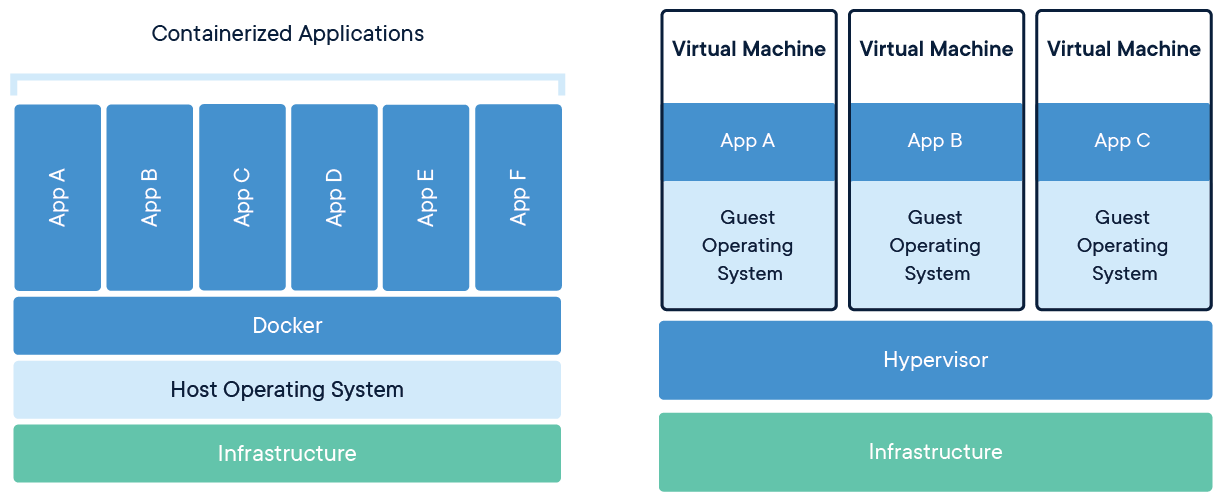
\includegraphics[width=\textwidth]{assets/dockerdiagram.png}
\end{frame}
\note[itemize]{
  \item containerization not a VM; a virtual machine runs on a hypervisor which
    abstracts the kernel: I/O, scheduling, etc.
  \item containerization exposes the underlying kernel, but virtualizes
    userspace
}

\begin{frame}{Orchestration}
  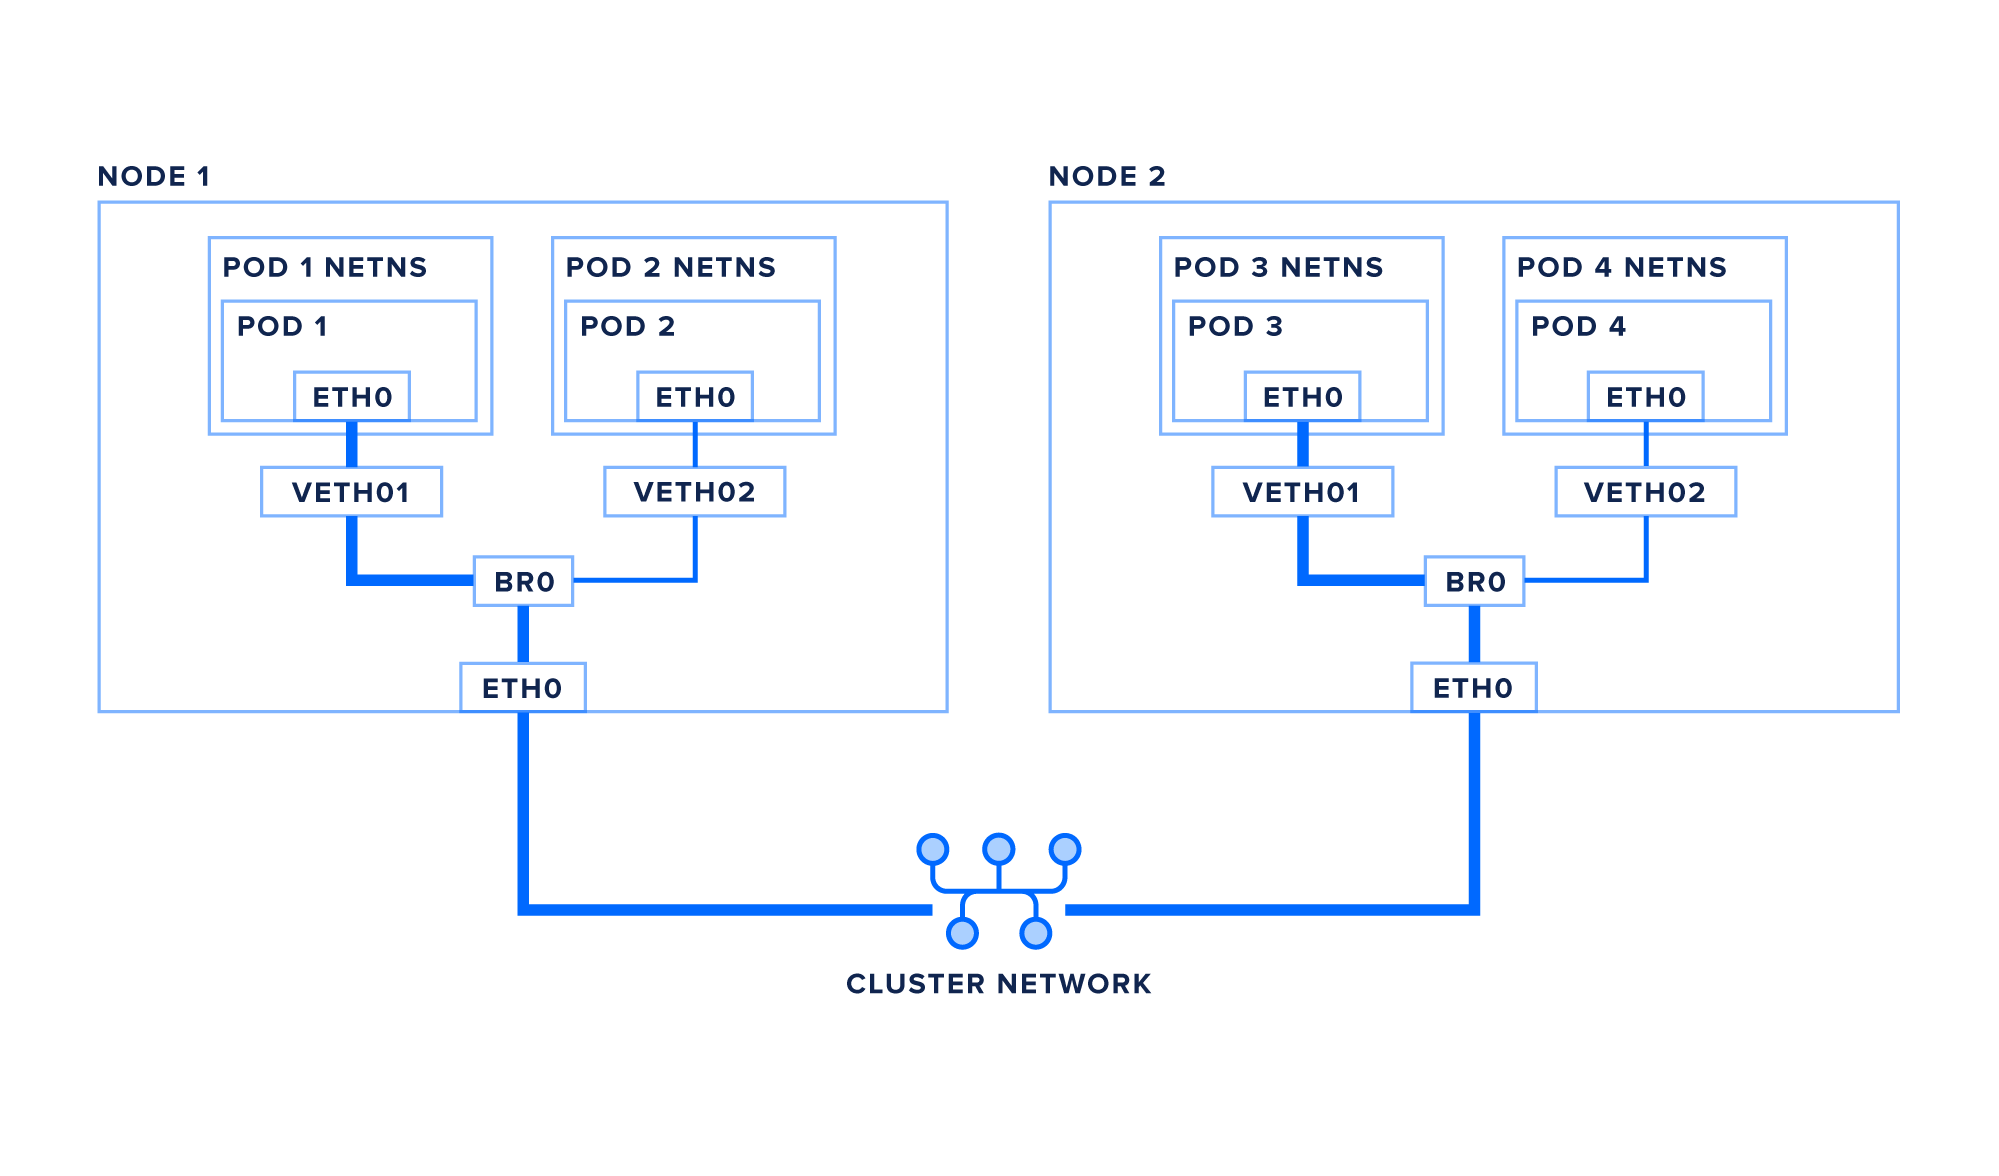
\includegraphics[width=\textwidth]{assets/kubenetwork.png}
\end{frame}
\note[itemize]{
  \item orchestration provides a declarative configuration of what services
    must be run, what service, how many instances
  \item orchestrators observe current state, and make it match configuration
  \item orchestrators also provide health checks, load balancing, service
    discovery, virtualized network, across hosts
}

\begin{frame}{Abridged History}
  \begin{description}
    \item[Mesos] 2009, distributed process manager
    \item[Docker] 2013, first to build an engine around Linux containers
    \item[Kubernetes] 2014, Google's solution to containerization with lessons
      learned from their internal Borg platform
  \end{description}
\end{frame}

\begin{frame}{Docker in Depth}
  \begin{itemize}
    \item containerization and orchestration platform
    \item build, run, publish containers
    \item deploy services with health checks
    \item provides virtualized network for container communication
    \item persistent state can be stored in volumes
    \item publicly available library of container images for services:
      PostgreSQL, Redis, Minio, etc.
    \item can test applications locally in the same environment as production
  \end{itemize}
\end{frame}
\note[itemize]{
  \item docker allows application to exist in a uniform environment whether
    local or in production
  \item allows scaling via declarative configuration
}

\begin{frame}
  \Huge DEMO
\end{frame}
\note[itemize]{
  \item creating an image with a Dockerfile
  \item running that image on any local port
  \item show and run docker swarm example
}

\section{Tooling}
\note[itemize]{
  \item command line is the de facto interface for developers
  \item cli has a learning curve
  \item important to know what tools exist to make QOL better
  \item here are a list of tools that make my life easier
}

\subsection{Command line}

\begin{frame}{SSH}
  \begin{itemize}
    \item Secure shell
    \item remote command line
    \item general cryptographic data transfer
    \item ssh tunnelling
    \item use ed25519 elliptic curve key pairs, 256 bits of randomness, with
      elliptic curve over a Galois field
    \item rsa4096 relies on prime number factors, thus not full 4096 bits of
      randomness
    \item ssh config
  \end{itemize}
\end{frame}
\note[itemize]{
  \item demo ssh tunnelling into database
}

\begin{frame}{tmux}
  \begin{itemize}
    \item screen multiplexer
    \item long running terminal sessions
    \item split a single terminal into panes, windows
  \end{itemize}
\end{frame}
\note[itemize]{
  \item demo creating panes and windows, reconnecting
}

\begin{frame}{watch}
  \begin{itemize}
    \item repeat a command after a specified number of seconds
    \item useful for monitoring status output
  \end{itemize}
\end{frame}
\note[itemize]{
  \item demo monitoring statistics from database
}

\begin{frame}{make \& inotify-tools}
  \begin{itemize}
    \item make is useful to create short commands for faster testing, and less
      memorization
    \item inotify-tools can watch a directory for changes, and execute a
      command on update
  \end{itemize}
\end{frame}
\note[itemize]{
  \item demo updating this presentation
}

\begin{frame}{vim}
  \begin{itemize}
    \item vi improved; vi was a visual mode for ex, which was a version of ed
      with extended functionality
    \item no shortcuts like other editors; uses text editing language with its
      own grammar
  \end{itemize}
\end{frame}

\section{Scaling}
\note[itemize]{
  \item paradigm remains largely the same across architectures
  \item goal is to route requests and responses from clients to servers
  \item what is the first scaling strategy?
}

\subsection{Optimization}

\begin{frame}{Caching}
  Client side
  \begin{itemize}
    \item HTTP Cache-Control headers
    \item ETag
    \item Last Modified
    \item hash filename, max-age 1 year
    \item service worker
  \end{itemize}
  Server side
  \begin{itemize}
    \item Redis \& Memcached
  \end{itemize}
\end{frame}
\note[itemize]{
  \item every bit that is cached client side is a bit that does not need to be
    transferred over the network
  \item cache control headers for static assets set by NGINX, or server
    middleware e.g. express.static
  \item hashing filename allows unchanged resources to be cached indefinitely
  \item otherwise using an etag and last modified will allow server to return
    304 Not Modified
  \item client caching increasingly necessary for mobile world
  \item server side cache reduces database load, db is often the source of
    bottlenecks
}

\begin{frame}{Numbers every programmer should know}
  \begin{itemize}
    \item L1 cache reference 0.5 ns
    \item Branch mispredict 5 ns
    \item L2 cache reference 7 ns
    \item Mutex lock/unlock 100 ns
    \item Main memory reference 100 ns
    \item Compress 1K bytes with Zippy 10,000 ns 0.01 ms
    \item Send 1K bytes over 1 Gbps network 10,000 ns 0.01 ms
    \item Read 1 MB sequentially from memory 250,000 ns 0.25 ms
    \item Round trip within same datacenter 500,000 ns 0.5 ms
    \item Disk seek 10,000,000 ns 10 ms
    \item Read 1 MB sequentially from network 10,000,000 ns 10 ms
    \item Read 1 MB sequentially from disk 30,000,000 ns 30 ms
    \item Send packet CA->Netherlands->CA 150,000,000 ns 150 ms
  \end{itemize}
  Jeff Dean
\end{frame}
\note[itemize]{
  \item network is just another leg of fetching information
  \item Jeff Dean, Numbers every programmer should know, given at Google
    Engineering All-Hands
}

\begin{frame}{Asset management}
  \begin{itemize}
    \item gzip, deflate all text: markup, scripts, styles, etc.
    \item often available by middleware e.g. compression for express
    \item do not compress images or video with the web server, they should
      already be compressed assets
    \item optipng -o7 -strip all input.png: losslessly compress png
    \item jpegtran -optimize -progressive -copy none input.jpg: optimize jpg
      DCT coefficients
    \item prefer jpg if no text
    \item jpg quality 85 recommended
    \item prefer mp4 over gif, gif has no temporal compression
    \item cache everything
  \end{itemize}
\end{frame}
\note[itemize]{
  \item better first load performance
  \item necessary for websites with large amounts of new data
  \item newer compression algorithms exist e.g. brotli, not well adopted
  \item boring is better
  \item how to handle increased load for dynamic data?
}

\subsection{Architecture}

\begin{frame}{Load Balancing}
  \begin{itemize}
    \item web servers can handle thousands of requests per second, normally not
      the bottleneck
    \item for more intensive workloads, can put a reverse proxy in front of
      multiple instances of the application server to distribute the load
    \item allows for automatic failover, high availability
  \end{itemize}
  \includegraphics[width=\textwidth]{loadbalance_gen.png}
\end{frame}
\note[itemize]{
  \item good for handling requests that need an immediate response
  \item app server is containerized so easy to scale
  \item popular load balancers are NGINX, HAProxy, Envoy, Traefik
  \item how to handle increased load for nonimmediate responses?
}

\begin{frame}{Architecture}
\end{frame}
\note[itemize]{
  \item load balancing
  \item service mesh
  \item message queue
  \item CDN
  \item edge computing
}

\end{document}
